\chapter{Kekul\'e \label{chap:kek}}

\begin{equation}
	u^{A,B}(\vec{r}_{A,B},t)=c \ e^{i \vec{r}_{A,B} \cdot \vec{K}} \label{eq:kek:displacements}
\end{equation}

\begin{figure}
	\begin{center}
	{
% Sizing constants
\newcommand{\alat}{1}
\newcommand{\amp}{.25}
\newcommand{\psize}{1 mm}
\newcommand{\sqth}{1.73205080757}

% Functions which draws the Kekule lattice
\newcommand{\kekdraw}[2]{
	\begin{scope}[xshift=#1*3.5 cm,yshift=-#2*3.5cm,scale=.4]

		%This scope is clipped to limit the drawn lattice to a square
		\clip (-3cm,-3cm) rectangle(3cm,3 cm);
		
		% Cycle through the lattice points
		\foreach \ip in {-2,-1,...,2}
			\foreach \im in {-2,-1,...,2}
			{
			% Draw the unkekuled lattice
			\node at ($\ip*\sqth*\alat/2*(1,{\sqth})+\im*\sqth*\alat/2*(-1,{\sqth})+(0,+\alat/2)$) [Au] {};
			\node at ($\ip*\sqth*\alat/2*(1,{\sqth})+\im*\sqth*\alat/2*(-1,{\sqth})+(0,-\alat/2)$) [Bu] {};

			% Draw the Kekuled lattice
			\node at ($\ip*\sqth*\alat/2*(1,{\sqth})+\im*\sqth*\alat/2*(-1,{\sqth})+(0,+\alat/2)
				+\amp*({cos(120*(\ip-\im)-30*(#1+1+3*#2))},{+sin(120*(\ip-\im)-30*(#1+1+3*#2))} )$)            [A] {};
			\node at ($\ip*\sqth*\alat/2*(1,{\sqth})+\im*\sqth*\alat/2*(-1,{\sqth})+(0,-\alat/2)
				+\amp*({cos(120*(\ip-\im)-30*(#1+1+3*#2))},{-sin(120*(\ip-\im)-30*(#1+1+3*#2))} )$)            [B] {};
			}

	\end{scope}
}

\begin{tikzpicture}[>=stealth,
		Bu/.style={circle,draw=blue!25,fill=blue!10,
			thick,minimum size=\psize,inner sep=0pt}, 					% Unkekuled A sublattice dots
		Au/.style={circle,draw=orange!35,fill=orange!20,
			thick,minimum size=\psize,inner sep=0pt},					% Unkekuled B sublattice dots
		B/.style={circle,draw=blue!50,fill=blue!20,
			thick,minimum size=\psize,inner sep=0pt}, 					% Kekuled A sublattice dots
		A/.style={circle,draw=orange!70,fill=orange!40,
			thick,minimum size=\psize,inner sep=0pt}]					% Kekuled B sublattice dots
		
		\foreach \itc in {-1,0,1}
			\foreach \itr in {0,1,...,3}
			{
				\kekdraw{\itc}{\itr}
				\pgfmathsetmacro\result{30*(\itc+1+3*\itr)};
				\node at (\itc*3.5 cm,-\itr*3.5cm+1.5cm) {$\omega t$=\pgfmathprintnumber[int trunc]{\result}};
			}
\end{tikzpicture}
}
	\end{center}
	\caption[]{}
\end{figure}

\section{Theory}
In this section the electronic band structure of the Kekul\'e lattice is calculated using a tight binding model for the expanded unit cell.
This calculation is done in two parts.
First, the effects of the change in lattice periodicity are discussed including a description of the zone folded electrical dispersion.
Second, it is shown that by perturbing the zone folded Hamiltonian the phonons gap the electronic dispersion.

\subsection{Kekul\'e geometry}
The Kekul\'e distortion causes an expansion of the unit cell, a reduction of the BZ, and a modification of the primitive lattice vectors and reciprocal lattice vectors.
When referencing the new geometry back to the intrinsic geometry, the notation previously developed in Chapter \ref{chap:TB} is used.
The expanded periodicity of the Kekul\'e lattice is determined by the periodicity of the distortion in Equation \ref{eq:kek:displacements}.
This term repeats whenever 
\begin{equation*}
	2 \pi=\vec{r}_{A,B} \cdot \bm{K}=(m \vec{a}_+ + n \vec{a}_-) \cdot (\vec{b}_+ - \vec{b}_-)/3=\frac{2 \pi}{3} (m-n) \ ,
\end{equation*}
resulting in the enlarged unit cell shown in Figure \ref{fig:kek:geometry}.

\begin{figure}
	\begin{center}
	% Comparing the Lattice and BZ with Kekule to without Kekule
{ % Scope so that user defined commands don't carry throughout
% Sizing constants
\newcommand{\alat}{1}
\newcommand{\amp}{.25}
\newcommand{\Klen}{2 cm}
\newcommand{\psize}{2 mm}
\newcommand{\sqth}{1.73205080757}

% Functions which draws the Kekule lattice
\newcommand{\kekdraw}{
	\begin{scope}

		%This scope is clipped to limit the drawn lattice to a square
		\clip (-3.9cm,-4.38cm) rectangle(3.9cm,3cm);
		
		% Cycle through the lattice points
		\foreach \ip in {-3,-2,...,3}
			\foreach \im in {-3,-2,...,3}
			{
			% Draw the unkekuled lattice
			\node at ($\ip*\sqth*\alat/2*(1,{\sqth})+\im*\sqth*\alat/2*(-1,{\sqth})+(0,+\alat/2)$) [Au] {};
			\node at ($\ip*\sqth*\alat/2*(1,{\sqth})+\im*\sqth*\alat/2*(-1,{\sqth})+(0,-\alat/2)$) [Bu] {};

			% Draw the Kekuled lattice
			\node at ($\ip*\sqth*\alat/2*(1,{\sqth})+\im*\sqth*\alat/2*(-1,{\sqth})+(0,+\alat/2)
				+\amp*({cos(120*(\ip-\im)-90)},{+sin(120*(\ip-\im)-90)} )$)            [A] {};
			\node at ($\ip*\sqth*\alat/2*(1,{\sqth})+\im*\sqth*\alat/2*(-1,{\sqth})+(0,-\alat/2)
				+\amp*({cos(120*(\ip-\im)-90)},{-sin(120*(\ip-\im)-90)} )$)            [B] {};
			}

	\end{scope}
}

\begin{tikzpicture}
	% Real space
	\begin{scope}[xshift=-3.75cm, scale=1,>=stealth,
		Bu/.style={circle,draw=blue!25,fill=blue!10,
			thick,minimum size=\psize,inner sep=0pt}, 					% Unkekuled A sublattice dots
		Au/.style={circle,draw=orange!35,fill=orange!20,
			thick,minimum size=\psize,inner sep=0pt},					% Unkekuled B sublattice dots
		B/.style={circle,draw=blue!50,fill=blue!20,
			thick,minimum size=\psize,inner sep=0pt}, 					% Kekuled A sublattice dots
		A/.style={circle,draw=orange!70,fill=orange!40,
			thick,minimum size=\psize,inner sep=0pt},					% Kekuled B sublattice dots
		nnarrow/.style={color=black,very thick, ->}]					% Arrows
		% Draw the lattice
		\kekdraw

		% Draw the primitive lattice vectors
		\draw[nnarrow] (0,-\alat*5/2) -- +( 30:3*\alat)node[anchor=south]{$\vec{A}_+$};
		\draw[nnarrow] (0,-\alat*5/2) -- +(150:3*\alat)node[anchor=south]{$\vec{A}_-$};

		% Draw the unit cell
		\draw[dashed,draw=black!75,rounded corners=.2cm,thick] (-\alat*\sqth*3/4,-\alat*15/4) rectangle (\alat*\sqth*3/4,-\alat*3/4);

	\end{scope}


	% Reciprical space
	\begin{scope}[xshift=3.75cm,yshift=-1 cm,scale=1,
		BZold/.style={color=black!75,very thick,dashed},
		BZnew/.style={color=black,very thick},
		Bar/.style={color=black,very thick,->},
		circ2/.style={radius=1.5pt}]

		% Draw the BZ
		\draw[BZold]
			(  0:\Klen) --
			( 60:\Klen) --
			(120:\Klen) -- 
			(180:\Klen) -- 
			(240:\Klen) -- 
			(300:\Klen) -- 
			(  0:\Klen);

					% Draw the BZ
		\draw[BZnew]
			( 30:\Klen/\sqth) --
			( 90:\Klen/\sqth) --
			(150:\Klen/\sqth) -- 
			(210:\Klen/\sqth) -- 
			(270:\Klen/\sqth) -- 
			(330:\Klen/\sqth) -- 
			( 30:\Klen/\sqth);

		\draw[Bar] (0,0) -- ( 60:\Klen) node[anchor=south west]{$\vec{B}_+$};
		\draw[Bar] (0,0) -- (120:\Klen) node[anchor=south east]{$\vec{B}_-$};

		% Label the high symmetry points
		\draw[fill=black] (0,0) circle[circ2] node[anchor=west]{$\Gamma$};
	\end{scope}
	\node at (-7cm,3.5cm) {\textbf{(a)}};
	\node at ( 1cm,3.5cm) {\textbf{(b)}};
\end{tikzpicture}
}
	\end{center}
	\caption[The geometry of the Kekul\'e lattice]{\label{fig:kek:geometry}
		The real space (a) and reciprocal space (b) geometry of the Kekul\'e lattice.
		Figure (a) shows a snapshot of the atomic positions with the A sub-lattice shown as orange dots and the B sub-lattice shown as blue dots.	
		For reference, the intrinsic graphene lattice is shown using faded dots.
		The dashed rectangle outlines the time independent unit cell and the labeled arrows represent the primitive lattice vectors.
		In (b) the hexagon with dashed lines indicates the BZ of intrinsic graphene while the hexagon with solid lines indicates the shrunken BZ of the Kekul\'e lattice.
		The primitive reciprocal lattice vectors are labeled.
	}
\end{figure}

The primitive lattice vectors of the Kekule\'e lattice,
\begin{align*}
	\vec{A}_+&=2 \vec{a}_+-\vec{a}_-=\frac{3 a}{2} (+\sqrt{3},1) \\
	\vec{A}_-&=2 \vec{a}_--\vec{a}_+=\frac{3 a}{2} (-\sqrt{3},1) \ ,
\end{align*}
represent a triangular lattice rotated by 90 degrees and expanded by a factor of $\sqrt{3}$ relative to the intrinsic lattice.
This tripling of the area of the unit cell is accompanied by a corresponding decrease in the area of the BZ as shown in Figure \ref{fig:kek:geometry}.
The primitive reciprocal lattice vectors,
\begin{align*}
	\vec{B}_+&=\frac{1}{3} (2\vec{b}_+ + \vec{b}_-)=\frac{2 \pi}{3 \sqrt{3} a}(+1,\sqrt{3}) \\
	\vec{B}_-&=\frac{1}{3} (2\vec{b}_- + \vec{b}_+)=\frac{2 \pi}{3 \sqrt{3} a}(-1,\sqrt{3}) \ ,
\end{align*}
generate a hexagonal BZ rotated 90 degrees and shrunken by a factor of three relative to the intrinsic lattice.
Unlike for intrinsic graphene, the interesting physics occurs near the center of the BZ.
For completeness, three equivalent corners of the BZ are positioned at
\begin{equation*}
	\frac{2 \pi}{9 a} (-\sqrt{3},-1), \ \ \frac{2 \pi}{9 a} (+\sqrt{3},-1), \ \ \textrm{and} \ \  \frac{2 \pi}{9 a} (0,2) \ .
\end{equation*}

\subsection{Zone folding}
When the BZ is reduced in size the two band dispersion of intrinsic graphene becomes a six band dispersion.
The energy bands outside the new BZ are folded into the new BZ by translation by a reciprocal lattice vectors.
Since the size of BZ is reduced by a factor there are two zone folding schemes resulting in six energy bands.

The zone folding schemes shown in Figure \ref{fig:kek:folding} describe the two distinct ways the symmetry reduced area of the new BZ can be mapped onto via translations of reciprocal lattice vectors.
The rest of the BZ can be constructed using symmetry operations on the symmetry reduced area.
In both zone folding schemes, the Dirac point is translated from the corner of the old BZ to the zone center.
Since this will still correspond to the charge neutrality point, this is the point in the new BZ we will be most interested in.
It is also worth noting that right edge of the symmetry reduced area in zone fold 1 shares its right edge with the symmetry reduced area already inside the new BZ.
Also, the top edge of the symmetry reduced area is shared between zone fold 1 and zone fold 2.

The hierarchy of the folded energy bands away from degeneracies can be determined by comparing the zone folded areas to the electronic dispersion of intrinsic graphene shown in Figure \ref{fig:TB:Dispersion}.
Just like for intrinsic graphene the the energy bands should be symmetric about the charge neutrality point.
The new BZ occupies the basin in the intrinsic graphene dispersion.
Thus, the unfolded area gives the lowest and highest energy bands.
Zone fold 1 extends further into the basin of intrinsic graphene's dispersion and so gives the second lowest and second highest energy bands.
Finally, the zone fold 2 gives the two middle energy bands.

\begin{figure}
	\begin{center}
	{
\newcommand{\Klen}{2 cm}
\newcommand{\sqth}{1.73205080757}
\newcommand{\BZ}{
	% Draw the old BZ
	\draw[BZold]
		(  0:\Klen) --
		( 60:\Klen) --
		(120:\Klen) -- 
		(180:\Klen) -- 
		(240:\Klen) -- 
		(300:\Klen) -- 
		(  0:\Klen);

	% Draw the new BZ
	\draw[BZnew]
		( 30:\Klen/\sqth) --
		( 90:\Klen/\sqth) --
		(150:\Klen/\sqth) -- 
		(210:\Klen/\sqth) -- 
		(270:\Klen/\sqth) -- 
		(330:\Klen/\sqth) -- 
		( 30:\Klen/\sqth);
}
\newcommand{\elemone}[2]
{
	\draw[fill=#1!30,draw=#1!90,rotate=#2] (0,0) -- (-30:\Klen/\sqth) -- (30:\Klen/\sqth) --cycle;
	\draw[fill=#1!30,draw=#1!90,rotate=#2,xshift=-\Klen] (0,0) -- (-30:\Klen/\sqth) -- (30:\Klen/\sqth) --cycle;
}

\newcommand{\elemtwo}[3]
{
	\draw[fill=#1!30,draw=#1!90,xscale=#3,rotate=#2]  (0,0) -- (\Klen/2,0) -- (30:\Klen/\sqth) --cycle;
	\draw[fill=#1!30,draw=#1!90,xscale=#3,rotate=#2,shift={(60:-\Klen)}] (0,0) -- (\Klen/2,0) -- (30:\Klen/\sqth) --cycle;
}

\begin{tikzpicture}[scale=1,
		BZnew/.style={color=black!90,thick},
		BZold/.style={color=black!90,thick,dashed},
		Bar/.style={color=black,thick,<-,>=stealth},
		circ2/.style={radius=1.5pt}]

	% Zone fold 1
	\begin{scope}[xshift=-2.5cm]

		% Draws the zones folding in
		\foreach \i/\colora in {0/{red},60/{blue},120/{green},180/{violet},240/{orange},300/{gray}} {
			\elemone{\colora}{\i}
		}

		% Draws on the old and new BZ
		\BZ

		% Draws the reduced symetric elemtn
		\draw[black] (0,0) -- (\Klen/2,0) -- (30:\Klen/\sqth) --cycle;
		\draw[black,xshift=-\Klen] (0,0) -- (\Klen/2,0) -- (30:\Klen/\sqth) --cycle;
		
		% Draws the arrow showing the shift in the reduced element
		\draw[Bar] (15:\Klen/\sqth/2*1.25) --node[above,xshift=.3cm]{$\vec{B}_+-\vec{B}_-$} ++(-\Klen,0);
	\end{scope}

	% Zone fold 2
	\begin{scope}[xshift=+2.5cm]

		% Draws the zones folding in
		\foreach \i/\colora in {0/{red},60/{blue},120/{green},180/{violet},240/{orange},300/{gray}} {
			\elemtwo{\colora}{\i}{1}
		}
		\foreach \i/\colora in {0/{yellow},60/{brown},120/{teal},180/{olive},240/{cyan},300/{magenta}} {
			\elemtwo{\colora}{\i}{-1}
		}

		% Draws on the old and new BZ
		\BZ

		% Draws the reduced symetric elemtn
		\draw[black] (0,0) -- (\Klen/2,0) -- (30:\Klen/\sqth) --cycle;
		\draw[black,shift={(60:-\Klen)}] (0,0) -- (\Klen/2,0) -- (30:\Klen/\sqth) --cycle;
		
		% Draws the arrow showing the shift in the reduced element
		\draw[Bar] ( 15:\Klen/\sqth/2*1.25) -- node[right]{$\vec{B}_+$} ++(240:\Klen);
	\end{scope}

	\node at (-3cm,2.5cm) {\textbf{(a) Zone Fold 1}};
	\node at (2cm,2.5cm) {\textbf{(b) Zone Fold 2}};
\end{tikzpicture}
}
	\end{center}
	\caption[The zone foldings introduced by the Kekul\'e distortion]{\label{fig:kek:folding}
		The zone foldings introduced by the Kekul\'e distortion.
		The outer hexagon with dashed lines is the BZ of intrinsic graphene and the inner hexagon with solid lines is the new BZ of the Kekul\'e lattice.
		Specifically shown, for both foldings the symmetry reduced area represented by the black outlined triangle is shifted by the labeled reciprocal lattice vector.
		}
\end{figure}

The zone folded electronic dispersion can either be calculated by folding the dispersion calculated in Chapter \ref{chap:TB} or by performing a tight binding calculation using the expanded unit cell.
Although it is more involved, the tight binding calculation will be done here because it will be needed later.
Each of the six atoms in the unit cell must have its own raising and lowering operator.
To simplify this bookkeeping the operators will be referenced back to the three two atom bases which make up the six atom Kekul\'e basis.
These two atom bases are shown in Figure \ref{fig:kek:hoppings}.
The operators $a_{i,l}$ and $b_{i,l}$ are then the lowering operators for the three A sub-lattice atoms and the three B sub-lattice atoms in the lth Kekul\'e basis respectively.
The index $i$ run over the three two atom bases.
In this notation the real space nearest neighbor tight binding Hamiltonian is given by
\newcommand{\rl}[4]{
	a^{\dagger}_{#1,#2} b_{#3,#4}
}
\begin{align}
	H=-\sum_l (
		 & t \rl{1}{l}{1}{l        }+t\rl{1}{l}{2}{l          }+t\rl{1}{l}{3}{l           } \nonumber \\
		+& t \rl{2}{l}{1}{l\uparrow}+t\rl{2}{l}{2}{l          }+t\rl{2}{l}{3}{l\rightarrow} \nonumber \\ 
		+& t \rl{3}{l}{1}{l\uparrow}+t\rl{3}{l}{2}{l\leftarrow}+t\rl{3}{l}{3}{l           } + \text{H.C.} ) \ .
		\label{eq:kek:Hreal}
\end{align}
Later the hopping energies $t$ will be made bond dependent to account for the altered nearest neighbor distances.
In the meantime the bond independent hopping energy of intrinsic graphene, $t_0$, will be used.

\begin{figure}
	\begin{center}
	{
\newcommand{\alat}{1}
\newcommand{\amp}{.075}
\newcommand{\psize}{2 mm}
\newcommand{\sqth}{1.73205080757}

% Functions which draws the Kekule lattice
\newcommand{\kekdraw}{
	\begin{scope}
		% Cycle through the lattice points
		\foreach \ip/\im in {0/0,1/0,0/1,-1/0,0/-1,-1/-1,-1/-2,-2/-1,-2/-2,1/-1,2/-2,1/-2,-1/1,-2/2,-2/1,0/-2,-2/0,-3/0,0/-3,1/-3,-3/1}
			{
			\node at ($\ip*\sqth*\alat/2*(1,{\sqth})+\im*\sqth*\alat/2*(-1,{\sqth})+(0,+\alat/2)
				+\amp*({cos(120*(\ip-\im)-90)},{+sin(120*(\ip-\im)-90)} )$)            [A] {};
			\node at ($\ip*\sqth*\alat/2*(1,{\sqth})+\im*\sqth*\alat/2*(-1,{\sqth})+(0,-\alat/2)
				+\amp*({cos(120*(\ip-\im)-90)},{-sin(120*(\ip-\im)-90)} )$)            [B] {};
			}

	\end{scope}
}
\begin{tikzpicture}[scale=.85,
		B/.style={circle,draw=blue!50,fill=blue!20,
			thick,minimum size=\psize,inner sep=0pt}, 					% Kekuled A sublattice dots
		A/.style={circle,draw=orange!70,fill=orange!40,
			thick,minimum size=\psize,inner sep=0pt},					% Kekuled B sublattice dots
		el1/.style={x radius=.3*\alat,y radius=.85*\alat},				% Style for the ellipse
		hops/.style={thick,black},										% Style for the hopping directions
		nnarrow/.style={color=black, ->,>=stealth}]						% Nearest neighbor vectors

	% Draw the hoppings we work with
	% \ip and \im specify the position of the A unit cell
	% \jp and \jm specify the position of the B unit cell
	\foreach \ip/\im/\jp/\jm in {-1/0/0/0,-1/0/-1/1,-1/0/-1/0,0/-1/0/0,0/-1/1/-1,0/-1/0/-1,-1/-1/-1/0,-1/-1/0/-1,-1/-1/-1/-1}{
		\draw[hops]
			($\ip*\sqth*\alat/2*(1,{\sqth})+\im*\sqth*\alat/2*(-1,{\sqth})+(0,+\alat/2)
			+\amp*({cos(120*(\ip-\im)-90)},{+sin(120*(\ip-\im)-90)} )$) -- 
			($\jp*\sqth*\alat/2*(1,{\sqth})+\jm*\sqth*\alat/2*(-1,{\sqth})+(0,-\alat/2)
			+\amp*({cos(120*(\jp-\jm)-90)},{-sin(120*(\jp-\jm)-90)} )$);
	}

	% Draw the atomic positions
	\kekdraw

	% Draw the Expanded units cells
	\foreach \Api/\Ami in {0/0,1/0,1/1,0/1,-1/0,-1/-1,0/-1}{
		\draw[dashed,draw=black!75,thick,shift={($\Api*3*\alat/2*(\sqth,1)+\Ami*3*\alat/2*(-\sqth,1)$)}]
			(-\alat*\sqth*3/4,-\alat*15/4) rectangle (\alat*\sqth*3/4,-\alat*3/4);
	}

	% Label the Expanded unit cells (only the ones we use)
	\foreach \Api/\Ami/\label in {0/0/$\bm{l}$,1/0/$\bm{l\rightarrow}$,1/1/$\bm{l\uparrow}$,0/1/$\bm{l\leftarrow}$}{
		\node at ($(-\alat*\sqth*3/4,-\alat*15/4)+\Api*3*\alat/2*(\sqth,1)+\Ami*3*\alat/2*(-\sqth,1)$) [anchor=south west] {\label} ;
	}

	% Draw the original unit cells
	% \foreach \api/\ami/\ind in {0/0/1,1/0/2,0/1/3,2/0/3,1/1/1,0/2/2}{
	% 	\draw[dashed,draw=black!75,thick,shift={($\api*\sqth*\alat/2*(1,{\sqth})+\ami*\sqth*\alat/2*(-1,{\sqth})$)}] 
	% 		(0,-3) ellipse[el1] node[xshift=.2cm] {$\bm{\ind}$};
	% }

	\foreach \api/\ami/\ind in {0/0/1,1/0/2,0/1/3,2/0/3,1/1/1,0/2/2}{
		\draw[dashed,draw=black!75,thick,
		shift={($\api*\sqth*\alat/2*(1,{\sqth})+\ami*\sqth*\alat/2*(-1,{\sqth})
				+\amp*({cos(120*(\api-\ami)-90)},0)$)}
		] 
			(0,-3) ellipse[el1] node[xshift=.125cm] {$\bm{\ind}$};

	% Draw the nearest neighbor vectors
	\draw[nnarrow] (6.5cm,-2cm) -- +(270:\alat) node[anchor=north     ]{$\vec{\delta}_1$};
	\draw[nnarrow] (6.5cm,-2cm) -- +( 30:\alat) node[anchor=south west]{$\vec{\delta}_2$};
	\draw[nnarrow] (6.5cm,-2cm) -- +(150:\alat) node[anchor=south east]{$\vec{\delta}_3$};
	}

\end{tikzpicture}
}
	\end{center}
	\caption[Diagram of the hoppings in the expanded Kekul\'e unit cell]{\label{fig:kek:hoppings}
		A diagram of the hoppings included in the Hamiltoninan.
		Hoppings connect atoms originally from the A sub-lattice (orange) to atoms originally from the B sub-lattice (blue).
		They can pass between the labeled intrinsic unit cells (dashed ellipses) and they can also pass between the labeled extended unit cells (dashed rectangles).
		For reference the directions of the nearest neighbor vectors are included.
	}
\end{figure}

Similarly to intrinsic graphene, the individual terms in the sum can be simplified by writing the operators in Fourier space,
\begin{equation}
	a_{m,l}^{\dagger}=\frac{1}{\sqrt{N}}\sum_{\vec{k}} e^{ i \vec{k}  \cdot \vec{R}_l} a_{m,\vec{k} }^{\dagger} \ ,
	\label{eq:kek:FT}
\end{equation}
where we are expanding about the positions of the Kekul\'e unit cells.
The individual terms are then
\begin{align*}
	-t_0 \sum_l \rl{m}{l}{m'}{l'} &=
	    -\frac{t_0}{N}\sum_l \sum_{\vec{k},\vec{k}'} \rl{m}{\vec{k}}{m'}{\vec{k}'} 
	    e^{i \vec{R}_l \cdot (\vec{k}-\vec{k}')} e^{i(\vec{R}_l-\vec{R}_l')\cdot \vec{k}'} \\
	    &= -t_0 \sum_{\vec{k}} \rl{m}{\vec{k}}{m'}{\vec{k}} \underbrace{e^{i(\vec{R}_l-\vec{R}_l')\cdot \vec{k}'}}_{s_{l-l'}} \ ,
\end{align*}
which is only dependent on the $l$ independent distance $l-l' \in \{ 0,\leftarrow,\uparrow,\rightarrow \}$ between the Kekul\'e unit cells that are being hopped between.

The Hamiltonian can then be expressed in matrix form as
\begin{equation}
	H_0=-t_0 \sum_{\vec{k}} \psi^{\dagger} 
	\left(\begin{array}{cccccc}
		0     & 0                 & 0                & s_0          & s_0            & s_0 \\
		0     & 0                 & 0                & s_{\uparrow} & s_0            & s_{\rightarrow} \\
		0     & 0                 & 0                & s_{\uparrow} & s_{\leftarrow} & s_0 \\
		s_0^* & s_{\uparrow}^*    & s_{\uparrow}^*   & 0            & 0              & 0 \\
		s_0^* & s_0^*             & s_{\leftarrow}^* & 0            & 0              & 0 \\
		s_0^* & s_{\rightarrow}^* & s_0^*            & 0            & 0              & 0 
	\end{array}\right)
	\psi \ ,
	\label{eq:kek:Hzonefold}
\end{equation}
where $\psi^{\dagger}=\left( a^{\dagger}_1, a^{\dagger}_2, a^{\dagger}_3, b^{\dagger}_1, b^{\dagger}_2, b^{\dagger}_3 \right)$.
As expected, the six by six Hamiltonian will provide six energy levels.

The zone folded electronic dispersion is shown in Figure \ref{fig:kek:zfdisp}.
To best show the shapes of the bands the dispersion is plotted both over the full Kekul\'e BZ and also over only the symmetry reduced area.
The six energy bands are clearly visible with the highest and lowest energy bands appearing as caps.
As expected the Dirac point has been shifted to zone center where the four lower energy bands converge to touch at a single point.
In agreement with the zone folding schemes the highest energy band is degenerate with the second highest energy band on the BZ border.
Also, the second and third highest energy bands are degenerate along the lines connecting the $\Gamma$ point to the BZ border.
In summary, the electronic dispersion calculated with a tight binding model of the expanded unit cell agrees with our zone folding predictions.

\begin{figure}
	\begin{center}
	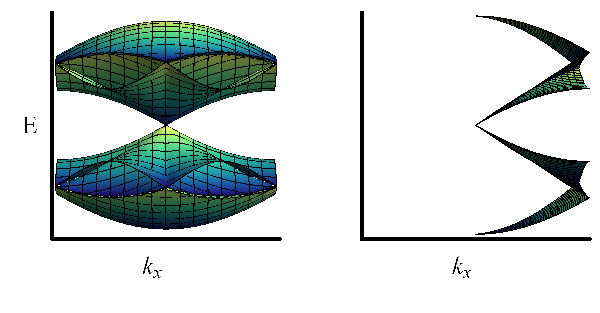
\includegraphics{Figs_Kekule/ZoneFolded.pdf}
	\end{center}
	\caption[Surface plots of the folded electronic dispersion of the Kekul\'e lattice]{\label{fig:kek:zfdisp}
		Surface plots of the folded electronic dispersion of the Kekul\'e lattice including all six energy bands.
		In the left plot the surfaces are plotted for the full Kekul\'e BZ whereas in the right plot only the symmetry reduced area is plotted.
	}
\end{figure}

\subsection{Altered hoppings}
Coherent excitation of the iTO phonon mode does more than just enlarge the unit cell, it also modifies the hopping energies.
This is similar to the case of strained graphene where the altered bond lengths caused altered hopping energies and generated new physics.
In this case, however, the bond lengths vary with a much higher spatial frequency and the slowly varying approximation described in Appendix \ref{chap:idep} is not applicable.
In fact, the atomic displacements in Equation \ref{eq:kek:displacements} will lead to hopping alterations with a spatial frequency of $\bm{G}=\bm{K}-\bm{K'}$
As mentioned in Appendix \ref{chap:idep}, a distortion with this frequency is expected to couple the inequivalent $\bm{K}$ and $\bm{K'}$ points.
This coupling will generate a band gap at the $\Gamma$ point of the zone folded dispersion.

Before determining the hopping alterations the bond length changes must be found.
Although it was helpful in finding the lengths of the strained nearest neighbor vectors in Section \ref{sub:PVP:straindistances}, the Cauchy-Born rule cannot be used here.
The iTO phonon causes the atoms in the A and B sub-lattices to rotate in opposite directions, an effect which an not be captured in the Cauchy-Born frame work.
Instead, the bond lengths must be calculated directly from the displacements.
Iadecola \textit{et al.} showed that the bond length alterations generate hopping alterations,
\begin{align}
	\delta t_{m,j}&=\frac{1}{3} \Delta(t) e^{i \bm{K} \cdot \vec{\delta}_j} e^{i \bm{G} \cdot \vec{r}_{m}}+\text{c.c.} \nonumber \\
	& \text{with } \Delta(t)=-i 3 \beta t_0 \frac{c^*}{a} e^{i \omega t} \label{eq:kek:hopps} \ ,
\end{align}
which have a spatial frequency component of $\bm{G}$ that couples the Dirac points \cite{Iadecola2013}.
Here $\vec{r}_{m}$ is the position of the A sub-lattice atom involved in the hopping.
Index $m$ indicates which of the three old unit cells the atom is in.
The B sub-lattice atom is specified through $\vec{\delta}_j$, the unperturbed nearest neighbor vector which connects the A sub-lattice atom to the B sub-lattice atom.
Figure \ref{fig:kek:hoppings} summarizes these indices.
For completeness, the calculation of Equation \ref{eq:kek:hopps} is included in Appendix \ref{chap:hopps}.

\subsection{Tight binding of the expanded Kekul\'e lattice}

The Kekul\'e mode causes the hopping energies in Equation \ref{eq:kek:Hreal} to be bond and time specific.
Taking $t=t_0+\delta t_{m,j}$ with $\delta t_{m,j}$ defined in equation \ref{eq:kek:hopps} breaks Equation \ref{eq:kek:Hreal} into two pieces.
The first, corresponding to $t_0$ is just the zone folding Hamiltonian in Equation \ref{eq:kek:Hzonefold}.
The second is the additional perturbation which opens the band gap.

Similar to the individual terms in $H_0$, each term in $H'$ can be simplified by writing the operators in Fourier using Equation \ref{eq:kek:FT} 
\begin{align*}
	- \sum_{l} \delta t_{m,j} \rl{m}{l}{m'}{l'} &= 
	    -\frac{1}{N}\sum_l \sum_{\vec{k},\vec{k}'} \delta t_{m,j} \rl{m}{\vec{k}}{m'}{\vec{k}'} 
	    e^{i \vec{R}_l \cdot (\vec{k}-\vec{k}')} e^{i(\vec{R}_l-\vec{R}_l')\cdot \vec{k}'} \\
	    &= \frac{1}{3}  \sum_{\vec{k}} \rl{m}{\vec{k}}{m'}{\vec{k}} 
	    	\underbrace{ \Delta (t) \left\{ e^{i \bm{K} \cdot \vec{\delta}_j} e^{i \bm{G} \cdot \vec{r}_{m}}+\text{c.c.} \right\} e^{i(\vec{R}_l-\vec{R}_l')\cdot \vec{k}}}_{g_{m,j,l-l'}} \ .
\end{align*}
In addition to the $l$ independent distance between involved Kekul\'e unit cells, each term depends on $m$ which indicates the old unit cell which the A sub-lattice atom occupies, and $j$ which indicates which $\vec{\delta}_j$ the hopping is along.
The associated vectors are $\vec{R}_l-\vec{R}_l' \in \{ 0, \vec{A}_+, \vec{A}_+ +\vec{A}_-,\vec{A}_- \}$ and $\vec{r}_m \in {0, \vec{a}_+,\vec{a}_-}$.

Figure \ref{fig:kek:hoppings} is useful in determining the elements of perturbed Hamiltonian.
\begin{equation*}
	H'=-\frac{1}{3} \sum_{\vec{k}} \psi^{\dagger} 
	\left(\begin{array}{cccccc}
		0           & 0                     & 0                    & g_{1,1,0}        & g_{1,2,0}          & g_{1,3,0} \\
		0           & 0                     & 0                    & g_{2,3,\uparrow} & g_{2,1,0}          & g_{2,2,\rightarrow} \\
		0           & 0                     & 0                    & g_{3,2,\uparrow} & g_{3,3,\leftarrow} & g_{3,1,0} \\
		g_{1,1,0}^* & g_{2,3,\uparrow}^*    & g_{3,2,\uparrow}^*   & 0            & 0              & 0 \\
		g_{1,2,0}^* & g_{2,1,0}^*           & g_{3,3,\leftarrow}^* & 0            & 0              & 0 \\
		g_{1,3,0}^* & g_{2,2,\rightarrow}^* & g_{3,1,0}^*          & 0            & 0              & 0 
	\end{array}\right)
	\psi \ ,
\end{equation*}

\subsection{Results and discussion}

\section{Experimental design}
\subsection{Phonon excitation}
\subsection{Band gap measurement}